\chapter{Background and Motivation}
\label{chap:background}

\section{Testing the Standard Model}
\section{Flavour Physics}
\subsection{The CKM Matrix}
\subsection{Weak Decays}

The key motivations for studying decays like the $B_s \to D_s l\nu$ are:
\begin{itemize}
	\item
	Determination of CKM matrix elements. Specifically, by combining the theoretical prediction and an observed brancing fraction of $B_s \to D_s l\nu$, $|V_{cb}|$ can be extracted.
	\item
	Precision tests of the standard model. There are currently a number of tensons between experiment and the standard model predictions of $B$ decays, some closely related to $B_s \to D_s l\nu$ \cite{Na:2015kha}.
\end{itemize}
We will first discuss the general ideas in computing semileptonic decays.
%-------------------------------------------------------------------------------------

%% {Semileptonic Decays}

\begin{wrapfigure}{R}{0.55\textwidth}
  \begin{center}
  \vspace{-25pt}
    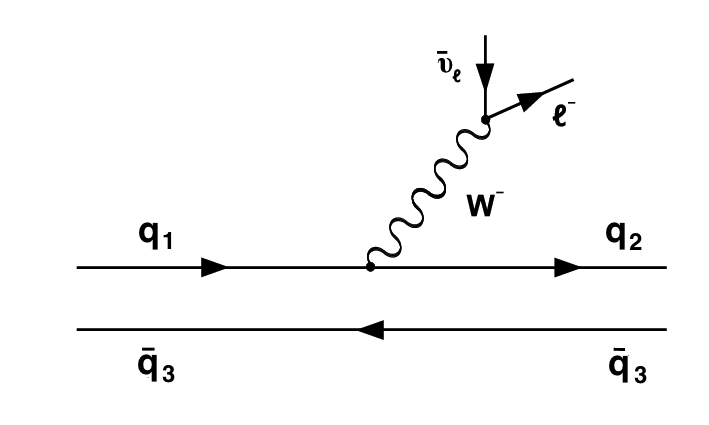
\includegraphics[width=
   0.5\textwidth]{images/semileptonic.png}
     \vspace{-25pt}
  \end{center}
  \caption{Semileptonic decay at tree level}
  \vspace{+10pt}
  \label{fig:semileptonic}
\end{wrapfigure}

Semileptonic decays are useful for studying the sector of the standard model (SM) which couples quarks to the weak force \cite{Richman:1995wm}:
\begin{align}
 \mathscr{L}_{W} & = {g\over\sqrt{2}} \left[ \quad V_{ij} J_{ij}^{\mu} W_{\mu}^+ + V^{\dagger}_{ij} J_{ij}^{\mu \dagger} W_{\mu}^- \quad \right]
  \label{eq:weakL}
\end{align}
$J_{\mu}^{ij} = \bar{u}_i \gamma_{\mu} {1\over2}(1-\gamma_5) d_j$ are the weak currents,
$\underline{u} = ( u, c, t )$ and $\underline{d} = ( d, s, b )$ are the quark fields, $g$ is the weak coupling constant, $W^{\pm}$ are the charged weak bosons, and $V$ is the (unitary)
Cabibbo-Kobayashi-Maskawa (CKM) matrix. $V_{ij}$ can be thought of as a matrix of couplings which dictate the probability
of mixing between two quark flavours, for example the amplitude of a $b$ decaying to a $u$ (and emitting a $W$) is proportional to $V_{13} \equiv V_{ub}$.
\\ \\
A semileptonic decay is any $hardon\to hadron+leptons$ process. Fig. \ref{fig:semileptonic} shows the tree level (in weak coupling) contribution to a semileptonic decay. We denote a meson with valence quark content $q$ and $q'$ as $M_{qq'}$. The $M_{q_1\bar{q}_3} \to M_{q_2\bar{q}_3} l \bar{\nu}_l$ decay ($l$ is some charged lepton and $\bar{\nu}_l$ is it's neutrino) is proportional to $V_{q_1q_2}$ at tree level.
\\ \\
This is given by
\begin{align}
  \mathcal{M} = \left({ig\over\sqrt{2}}\right)^2 V_{q_1q_2} \langle M_{q_2\bar{q}_3}, l\bar{\nu} | J_{\alpha}^{q_1\bar{q}_2} D^{\alpha\beta}_W(p^2) J^{l\bar{\nu}}_{\beta} | M_{q_2\bar{q}_3} \rangle
\end{align}
$J^{l\bar{\nu}}$ is the analog of the quark currents $J^{q_1\bar{q}_2}$, since the $W$ couples in the same way to leptons (with $V$ replaced by a unit matrix).
If the external momenta of the process $p^2$ are much smaller than the $W$ mass, one can remove the $W$ propagator from the tree level amplitude \cite{Borasoy:2007yi};
\begin{align}
 \left({ig\over\sqrt{2}}\right)^2 D^{\mu\nu}_W(p^2) = \left({ig\over\sqrt{2}}\right)^2 \left( -ig^{\mu\nu} \over p^2 - M_W^2 \right)
  & = \underbrace{ {i\over M_W^2} \left( ig \over \sqrt{2} \right)^2  }_{\equiv -2\sqrt{2}G_F} g^{\mu\nu} + \mathcal{O}\left({p^2\over M_W^4}\right)
\end{align}
Then $\mathcal{M}$ can be factorised;
\begin{align}
  \nonumber
  \mathcal{M} & \simeq -2\sqrt{2} G_F V_{q_1q_2} \langle M_{q_1\bar{q}_3}, l\bar{\nu} | J_{\mu}^{q_1\bar{q}_2} J^{l\bar{\nu} \mu} | M_{q_2\bar{q}_3} \rangle \\
  \nonumber
  & = -2\sqrt{2} G_F V_{q_1q_2} \langle l\bar{\nu} | J^{l\bar{\nu} \mu} | 0 \rangle \langle M_{q_1\bar{q_3}} | J_{\mu}^{q_1\bar{q}_2} | M_{q_2\bar{q}_2} \rangle \\
  & \equiv -2\sqrt{2} V_{q_1q_2} G_F L^{\mu} H_{\mu}.
  \label{eq:LH}
\end{align}
$L_{\mu}$ can be computed in perturbation theory. The hadronic matrix element $H_{\mu}$ however, due to the non-perturbative nature of QCD at low energies,
cannot be computed analytically. It is quantities such as $H_{\mu}$ that we wish to calculate in lattice QCD.

%% {CKM Extraction}

Speaking heuristically, if one can calculate the quantity $G_F L^{\mu} H_{\mu}$ from theory, and measures the amplitude of the process $\mathcal{M}$, they could then rearrange equation \eqref{eq:LH} to deduce $V_{q_1q_2}$. Speaking more practically, the relevant equation is, for example, for the $B_s \to D_s l\nu$ decay \cite{Na:2015kha}:
\begin{align}
	{d\Gamma \over dq^2} =& \eta_{\text{EW}} {G^2_F |V_{cb}|^2 \over 24\pi^3 M_{B_s}^2} \left( 1 - {m_l^2\over q^2}\right)^2 |\underline{p}| \\
	&\times \left[ \left(1+{m_l^2\over 2q^2}\right) M_{B_s}^2 |\underline{p}| f^2_+(q^2) + {3m_l^2\over 8q^2}(M_{B_s}^2 - M_{D_s}^2)^2 f_0^2(q^2)\right]
\end{align}
where $m_l$ is the mass of the charged lepton, $\eta_{\text{EW}}$ is an electroweak correction factor, $q^2$ is the momentum transfer, ${d\Gamma/dq^2}$ is the branching fraction, and $f_{0,+}(q^2)$ are the form factors associated with the decay, to be defined in \ref{sec:formfactors}. Given experimental data for ${d\Gamma/dq^2}$ and theoretical data for $f_{0,+}(q^2)$, one can deduce $|V_{cb}|$.
\\ \\
What is the value of determining CKM elements? Firstly, uncertainty in CKM elements are the dominant error in many standard model predictions. $V$ elements can also test the standard model. $V$ is unitary by definition. However, if there were more than 3 generations of quark, requiring $V$ to be 4x4 or larger, the 3x3 submatrix which couples the 3 known generations
would not itself be unitary in general (\cite{Schwartz:2013pla} ch. 29). Therefore, if one can deduce the elements of the 3x3 $V$ to high enough precision to show it is not unitary, this would be indirect evidence for new physics. 
\\ \\
Unitarity imposes a constraint on each row of $V$. The current status of the unitarity of $V$ can be read off from below (each quantity should be zero for unitarity to hold)\cite{Aoki:2016frl}:
\begin{align}
	\nonumber
	&|V_{ud}|^2 + |V_{us}|^2 + |V_{ub}|^2 - 1 = -0.020(9) \\ 
	&|V_{cd}|^2 + |V_{cs}|^2 + |V_{cb}|^2 - 1 = 0.06(3)
\end{align}
both of the above relations display a $\sim2\sigma$ deviation from unitarity. More precise values of these parameters are needed to discover if CKM is infact non-unitary.
\\ \\
Now we consider $|V_{cb}|$ specifically. $|V_{cb}|$ is the dominant uncertainty in many standard model predictions of rare decays, such as $B_s \to \mu^+\mu^-$,$K\to\pi\nu\bar{\nu}$, and the CP violation parameter $\epsilon_K$ \cite{Na:2015kha}. The FLAG working group quotes their average $|V_{cb}|$ to currently be \cite{Aoki:2016frl}:
\begin{align}
	|V_{cb}| = 0.04085(95)
\end{align}
However, the water is slightly muddied by the presence of tensions between different determinations of $|V_{cb}|$, namely between that deduced from studying $B\to D^*l\nu$, and an inclusive analysis of $B\to X_c l\nu$ where $X_c$ is any meson containing a $c$ quark \cite{Na:2015kha}:
\begin{align}
	|V_{cb}|_{\text{inclusive}} = 0.04221(78) \text{ , } |V_{cb}|^{B\to D^* l\nu} = 0.03904(49)_{\text{expt.}}(53)_{\text{QCD}}(19)_{\text{QED}}
\end{align}
A recent review of $|V_{cb}|$ determinations from the lattice is given in \cite{Wingate:2017unz}. This issue would benefit from a $|V_{cb}|$ determination from annother channel, like $B_s\to D_s l\nu$, to flesh out the landscape of $|V_{cb}|$ values and pinpoint the source of the tension, if there is any.

\subsection{Flavour Anomalies}

There are a number of tensions currently between theory and experiment in $B$ decays, who's true nature can be eludicated by our $B_s\to D_s l\nu$ study, and eventual $B\to Dl\nu$ study.
\\ \\
Define the ratios
\begin{align}
	R(X) = {\mathcal{B}(B\to X \tau \nu_{\tau}) \over \mathcal{B}(B\to X l \nu_l)}
\end{align}
where $l=e$ or $\mu$. These can be computed either purely from a lattice calculation, or purely from experimental data, independantly of the associated CKM element. It therefore can be used for comparison between experiment and the standard model. $R(D^*)$ contains a $~2.1\sigma$ discrepancy \cite{Aaij:2015yra}:
\begin{align}
	R(D^*)|_{\text{SM}} = 0.252(3) \text{ , } R(D^*)|_{\text{LHCb}} = 0.336(27)_{sys}(30)_{stat}
\end{align}
The issue is similarly present for $R(D)$ \cite{Monahan:2017uby}:
\begin{align}
	R(D)|_{\text{SM}} = 0.299(7) \text{ , } R(D)|_{\text{exp}} = 0.391(28)_{sys}(41)_{stat}
\end{align}
where in this case $R(D)|_{\text{expt}}$ is a world average of experimental values. Our eventual study of $B\to Dl\nu$ will produce a new standard model determination of $R(D)$, helping shed light on the issue.
\\ \\
\begin{figure}
  \begin{center}
    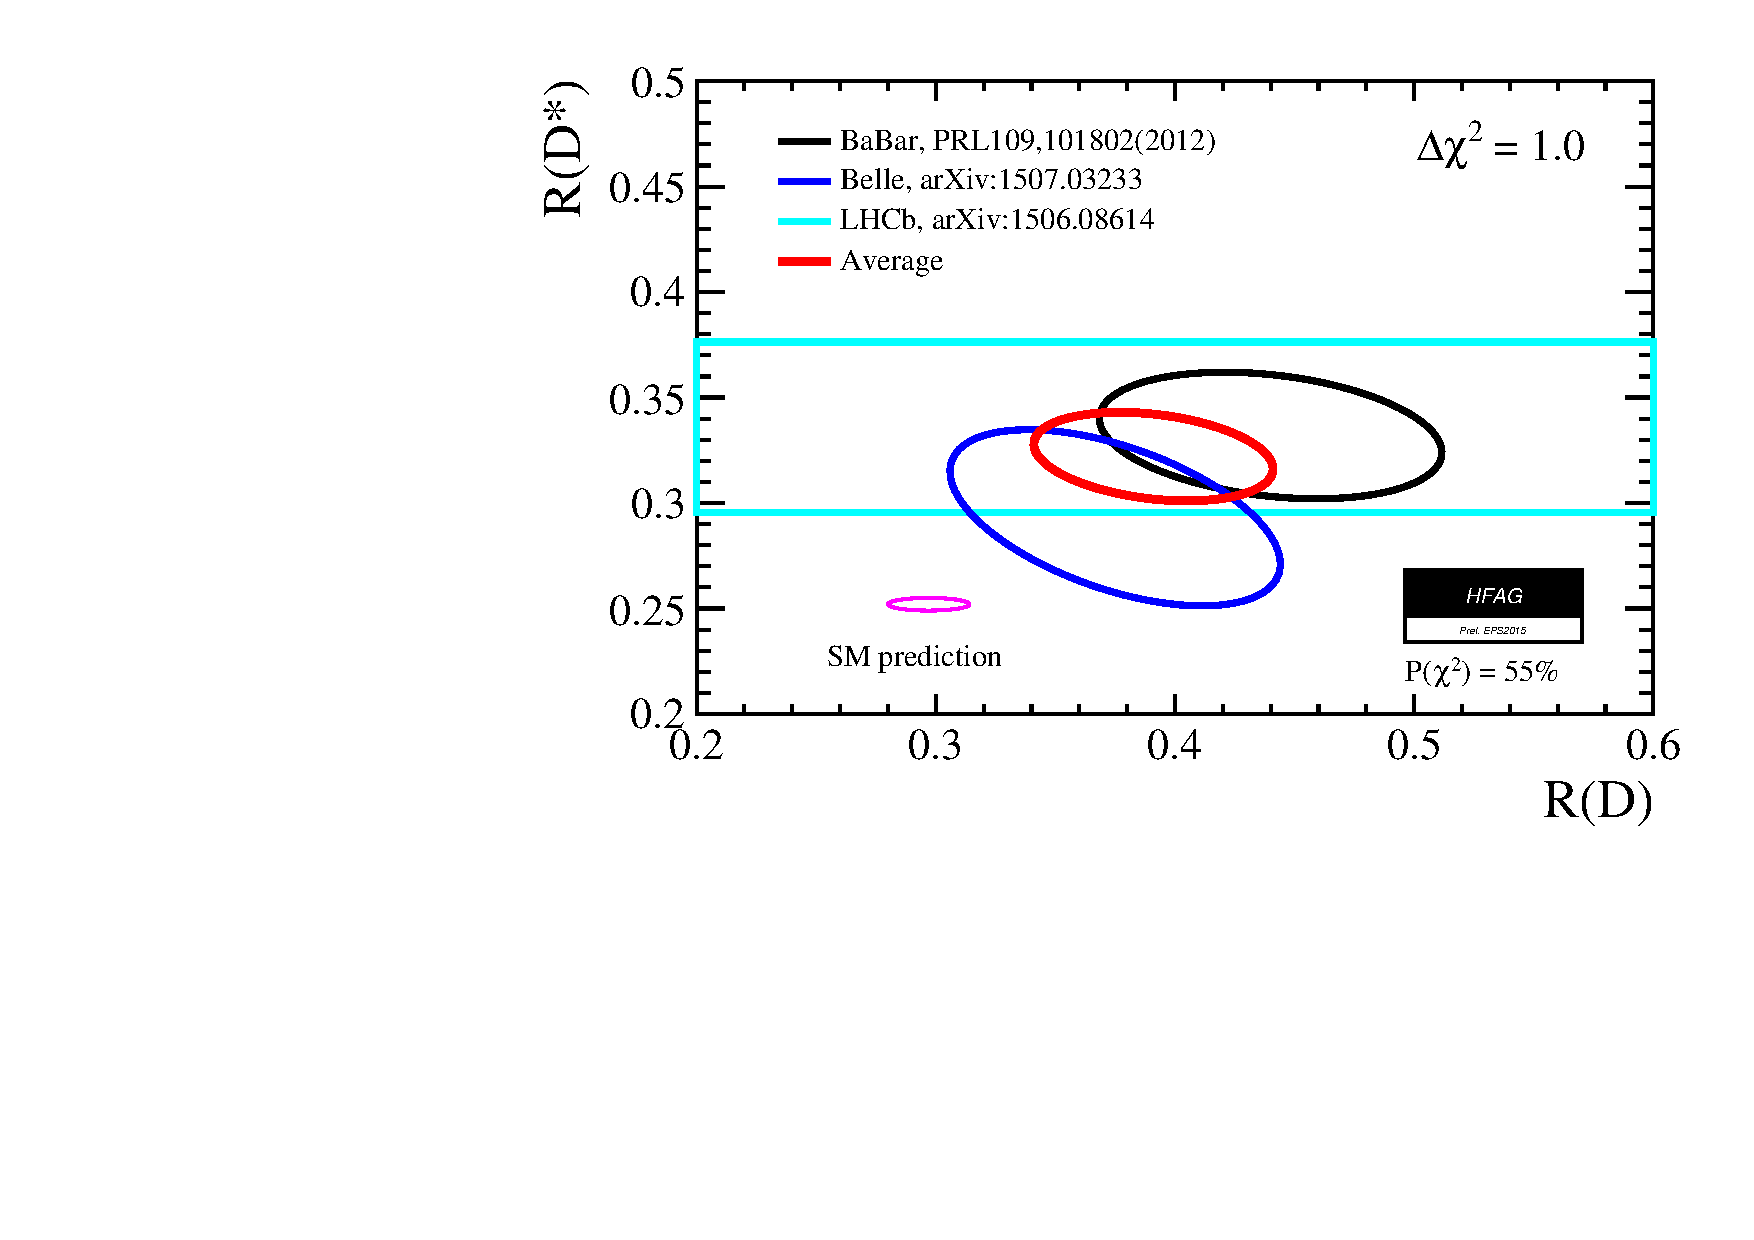
\includegraphics[width=
   0.8\textwidth]{images/rdrds_eps15.pdf}
  \end{center}
  \caption{$R(D)/R(D^*)$ determinations from standard model and experiment \cite{HFAG}}
  \label{fig:semileptonic}
\end{figure}
%A natural question to ask is: is there an analagous tension in related channels, like $B_s\to D_s l\nu$? There is not yet any experimental data for this decay, but the current best standard model determination is given by ${\mathcal{B}(B_s\to D_s \tau \nu_{\tau}) / \mathcal{B}(B_s\to D_s l \nu_l)} |_{\text{SM}} = 0.314(6)$.
\\ \\
Besides these, there are also tensions in the quantitites \cite{Altmannshofer:2017yso}:
\begin{align}
	R'(K^{(*)}) = {\mathcal{B}( B\to K^{(*)}\mu^+\mu^-)\over \mathcal{B}( B\to K^{(*)} e^+e^-)}
\end{align}
All of the above anomalies are suggestive of lepton flavour violating effects. Various BSM models have been suggested; hot topics include Leptoquarks, $Z'$ models, and partial compositeness \cite{Altmannshofer:2017yso}.

\subsection{Lepton Flavour Violation}
